\documentclass[12pt]{article}
\usepackage[letterpaper,margin=0.75in]{geometry}
\usepackage{graphicx}
\usepackage{setspace}
\usepackage{times}
\usepackage{array}
\usepackage{tabularx}
\usepackage{booktabs}
\usepackage{caption}
\usepackage{subcaption}
\usepackage{float}
\usepackage{amsmath}
\usepackage{amssymb}
\usepackage{enumitem}
\usepackage{titlesec}
\usepackage{tikz}
\usetikzlibrary{shapes.geometric, arrows.meta, positioning, calc, backgrounds, fit}
\usepackage[section]{placeins} % figures/tables cannot float past the next \section
\usepackage[hidelinks]{hyperref}

% ---------------- Spacing and layout ----------------
\doublespacing
\setlength{\parindent}{0.5in}
\setlist{nosep,topsep=2pt}

\titleformat{\section}{\normalfont\large\bfseries}{\thesection}{0.6em}{}
\titlespacing*{\section}{0pt}{8pt}{2pt}

\titleformat{\subsection}{\normalfont\normalsize\bfseries}{\thesubsection}{0.5em}{}
\titlespacing*{\subsection}{0pt}{6pt}{2pt}

\setlength{\abovedisplayskip}{3pt}
\setlength{\belowdisplayskip}{3pt}
\setlength{\abovedisplayshortskip}{0pt}
\setlength{\belowdisplayshortskip}{2pt}

\setlength{\floatsep}{6pt plus 2pt minus 2pt}
\setlength{\textfloatsep}{8pt plus 2pt minus 2pt}
\setlength{\intextsep}{8pt plus 2pt minus 2pt}
\renewcommand{\topfraction}{0.9}
\renewcommand{\bottomfraction}{0.9}
\renewcommand{\textfraction}{0.08}
\renewcommand{\floatpagefraction}{0.8}

\captionsetup{font={it,small},labelsep=space,skip=3pt}
\captionsetup[subfigure]{font={it,footnotesize},skip=2pt}
\renewcommand{\thefigure}{\arabic{section}.\arabic{figure}}
\makeatletter
\@addtoreset{figure}{section}
\makeatother

\begin{document}

% ---------------- Title block and cover table ----------------
\begin{flushleft}
\singlespacing
Yashwardhan Panchal\\
CSCI 5561 - Computer Vision\\
November 14, 2026\\[0.5em]
\begin{center}
\textbf{\Large HW3 Report}
\end{center}
\end{flushleft}

\begin{table}[H]
\centering
\singlespacing
\normalsize
\renewcommand{\arraystretch}{1.5}
\begin{tabularx}{\textwidth}{|X|c|c|c|}
\hline
\textbf{Assignment item} & \textbf{Points} & \textbf{Location in report} & \textbf{Extra credit?} \\
\hline
Report Quality & 10 & - & No \\
\hline
Gather Photographs & 10 & Section~\ref{sec:gather_photos}, p.~\pageref{sec:gather_photos} & No \\
\hline
Estimate Camera Parameters & 10 & Section~\ref{sec:camera_params}, p.~\pageref{sec:camera_params} & No \\
\hline
Two-Image 3D Reconstruction with SVD & 15 & Section~\ref{sec:svd_reconstruction}, p.~\pageref{sec:svd_reconstruction} & No \\
\hline
Multi-Image Reconstruction with COLMAP & 15 & Section~\ref{sec:colmap}, p.~\pageref{sec:colmap} & No \\
\hline
Gaussian Splatting & 15 & Section~\ref{sec:gaussian_splatting}, p.~\pageref{sec:gaussian_splatting} & No \\
\hline
% --- Additional Features (Select any combination totaling >= 25 pts) ---
Triangulation Refinement & 10 & Section~\ref{sec:triangulation_refinement}, p.~\pageref{sec:triangulation_refinement} & No \\
\hline
Learned Matching & 10 & Section~\ref{sec:learned_matching}, p.~\pageref{sec:learned_matching} & No \\
\hline
Held-Out View Evaluation & 10 & Section~\ref{sec:heldout_evaluation}, p.~\pageref{sec:heldout_evaluation} & Yes \\
\hline
% Artistic Reconstruction & - & Appendix~\ref{app:artistic}, p.~\pageref{app:artistic} & Bonus \\
% \hline
\textbf{Total attempted before extra-credit conversion} & \textbf{110} & & \\
\hline
\textbf{Maximum possible score after conversion} & \textbf{105} & & \\
\hline
\end{tabularx}
\caption*{Cover Page: Feature and Rubric Accounting Table}
\end{table}

\vfill
\clearpage

% ---------------- Introduction ----------------
\section*{Introduction}

% TODO: Brief high-level project summary:
% - Scene captured and reconstruction goal.
% - Connecting two-view epipolar geometry, SVD triangulation, multiview SfM (COLMAP), and 3D Gaussian Splatting.
% - Hardware/environment overview.

[Introduction text to be added here]


% ---------------- Section 1: Gather Photographs ----------------
\section{Gather Photographs}\label{sec:gather_photos}

% TODO: Describe:
% 1. Scene description and photography strategy (texture, depth variation, camera motion path).
% 2. Camera settings (focal length, sensor/lens, fixed focus/exposure, resolution, downsampling if any).
% 3. Selected image pair for two-view triangulation and justification (baseline, visual overlap, feature count).

The scene here is the center table in the living room of my apartment. 
I placed multiple objects on the table with different colors, shapes and depths to get a good reconstruction 
My stratergy was to capture the table from all 4 sides, cover wide range of angles. 
I captured photos from the top view as well as some close to the objects.

Iphone 17 main camera used. 40 photos captured initially but deleted two due to motion blur. Total images now are 38.
Original resolution of photos was 4284x5712. 
I shared it over Whatsapp to myself which automatically downsampled the images to 1200x1600.
I am using \texttt{image\_27.jpg} and \texttt{image\_29.jpg} for two-view reconstructions. The camera in \texttt{image\_27.jpg} sits in front of the camera in \texttt{image\_29.jpg}.
There is a lot of feature overlap and also covers the objects in scene from different angles, which is useful.

\begin{figure}[!htbp]
\centering
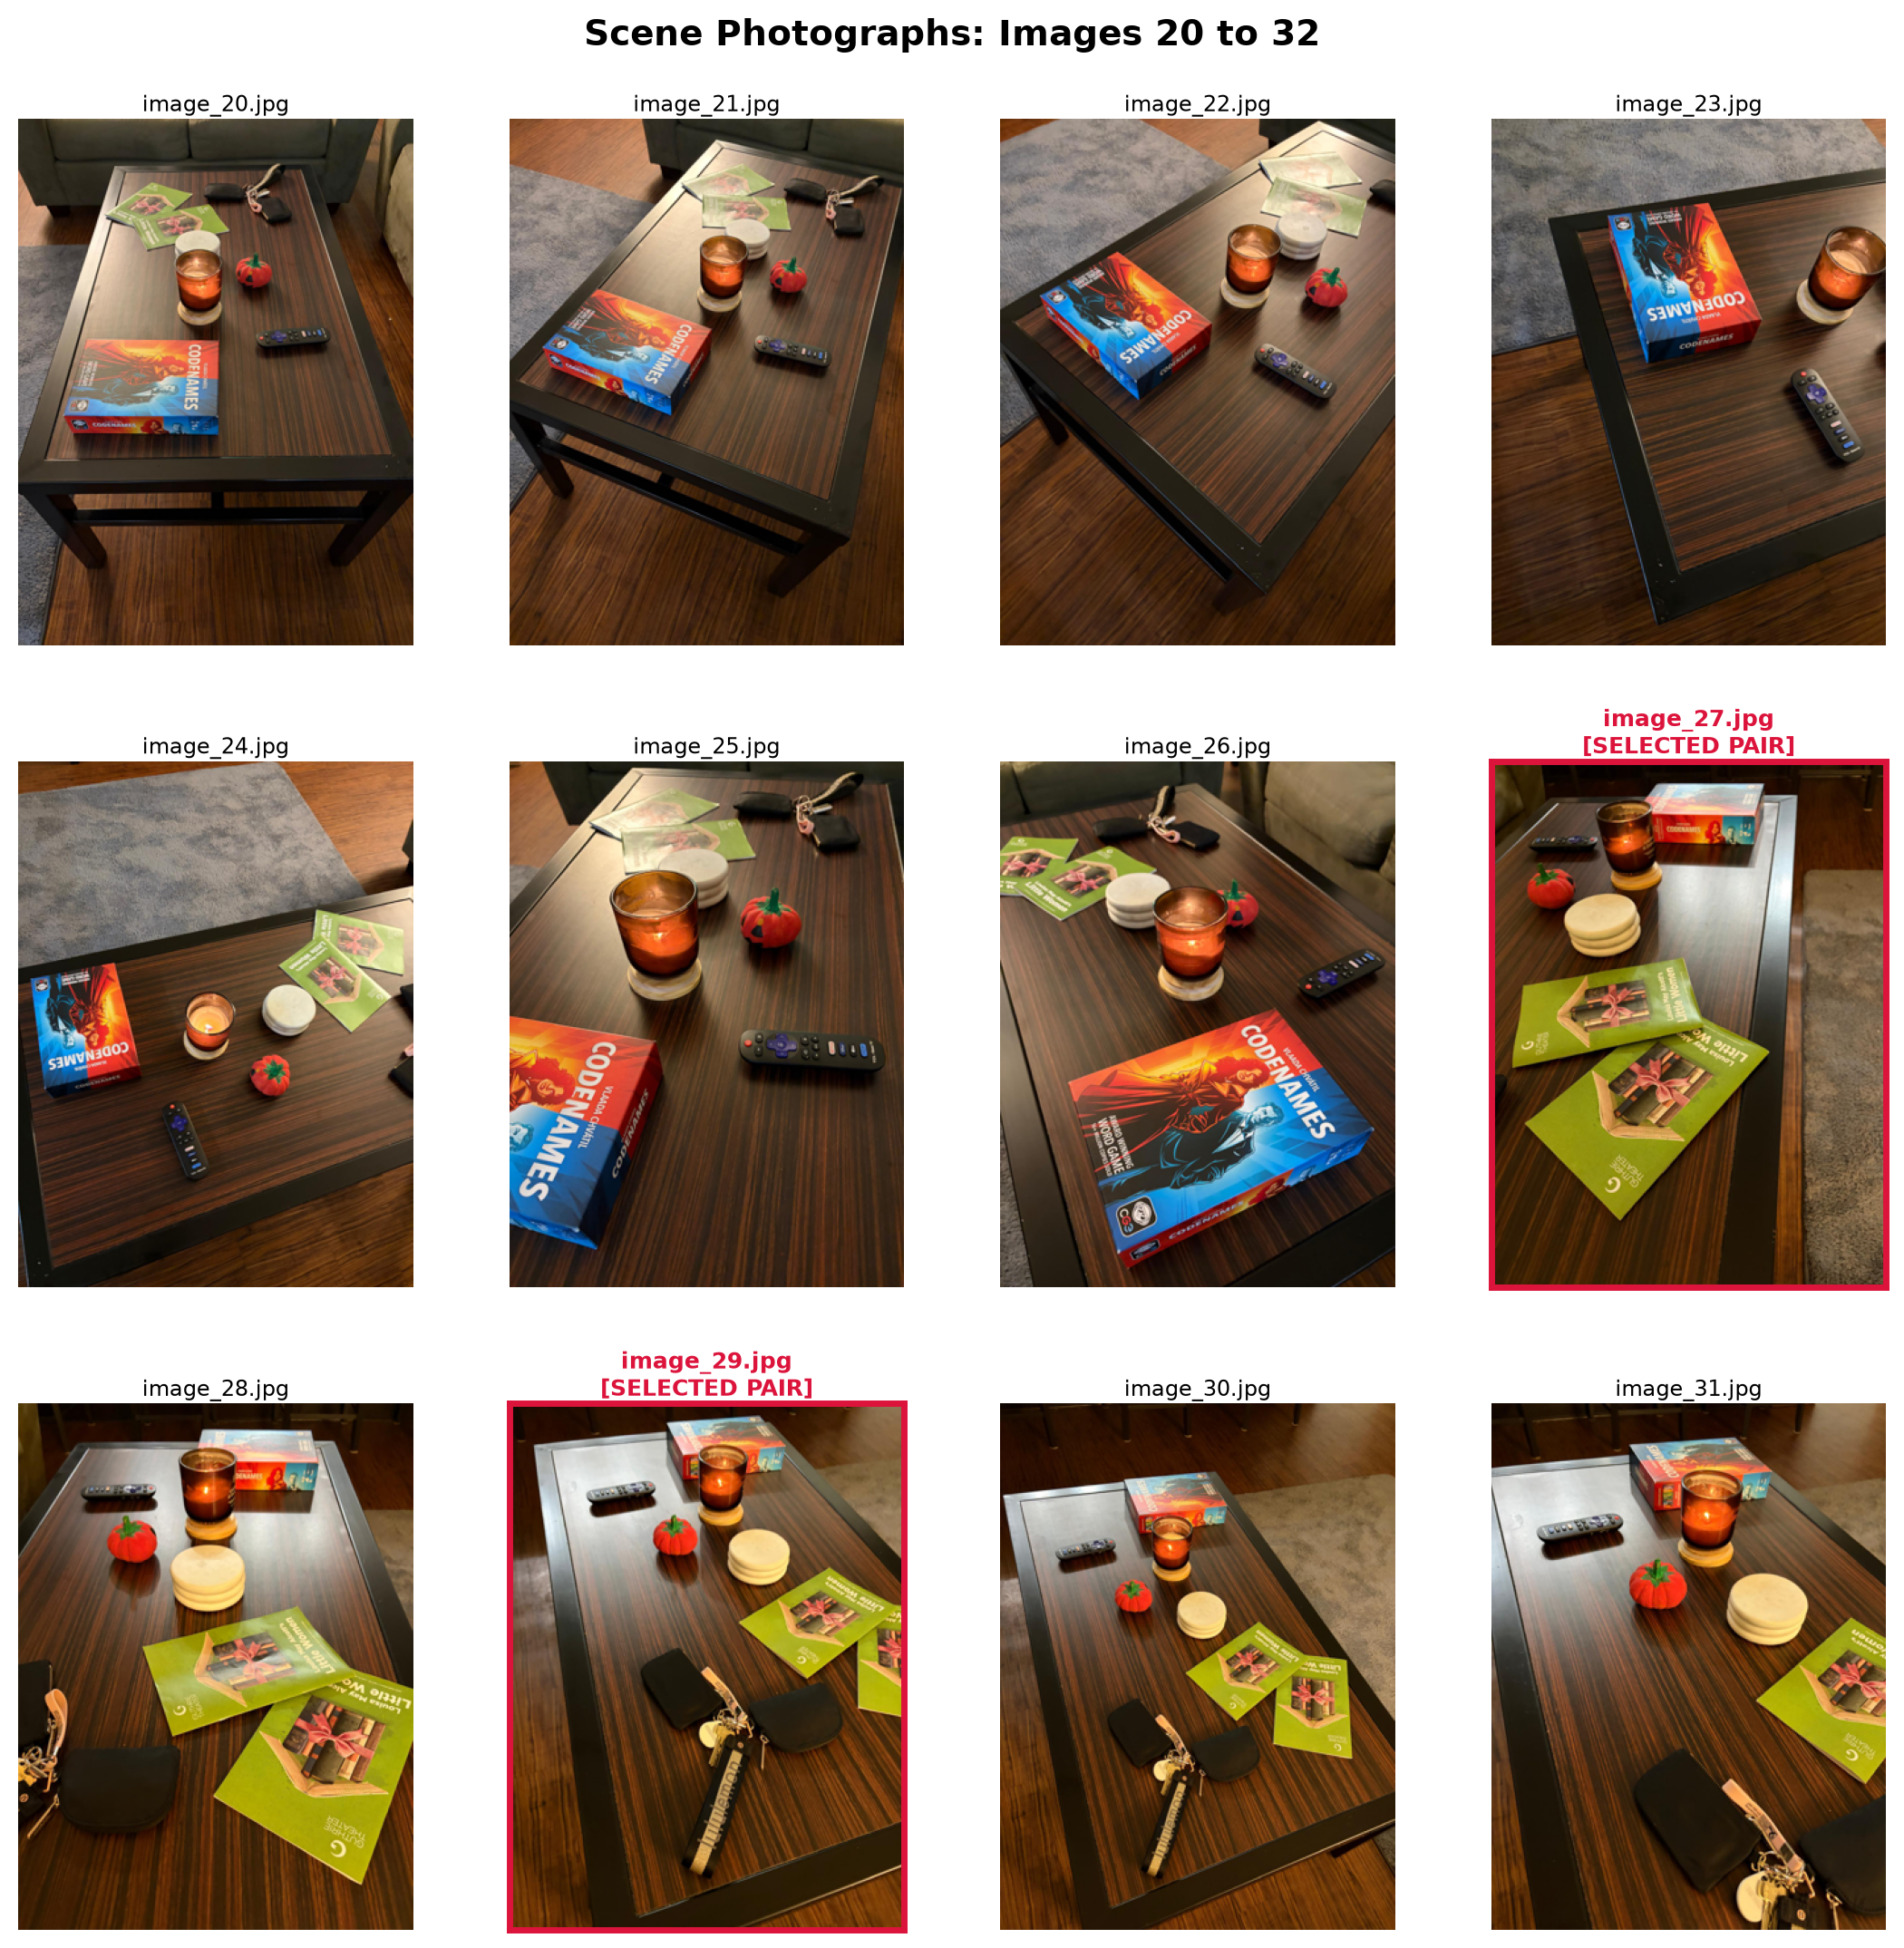
\includegraphics[width=0.9\textwidth]{figures/images_20_to_32_grid.png}
% \fbox{\rule{0pt}{2in}\rule{0.9\textwidth}{0pt}} % Placeholder box
\caption{Representative photographs from the captured scene collection, highlighting the selected image pair used for two-view triangulation and views demonstrating coverage and overlap.}
\label{fig:representative_photos}
\end{figure}


% ---------------- Section 2: Estimate Camera Parameters ----------------
\section{Estimate Camera Parameters}\label{sec:camera_params}

% TODO: Describe:
% 1. Source and derivation of intrinsic matrix K and lens distortion parameters.
% 2. SIFT feature detection and ratio-test matching on the selected pair.
% 3. Undistortion process (undistorted pixel vs. normalized coordinates).
% 4. Essential/Fundamental matrix estimation with RANSAC.
% 5. Relative pose recovery (R and unit translation t) and projection matrices P1 = K[I | 0], P2 = K[R | t].
% 6. Numerical values of E/F, R, t, match count, and inlier count.

To get the camera parameters for \texttt{image\_27.jpg} and \texttt{image\_29.jpg}, I used PyCOLMAP to find the camera intrinsics across my photo set, and then used OpenCV to estimate the relative pose between the two selected views.

\subsection{Camera Intrinsics from Multiview Reconstruction}
I estimated the camera intrinsic parameters from all 38 photos using PyCOLMAP (v3.13.0) with the \texttt{SIMPLE\_RADIAL} camera model. This model assumes a single shared pinhole camera with parameters $(f, c_x, c_y, k_1)$, where $f$ is focal length, $(c_x, c_y)$ is the principal point, and $k_1$ is radial distortion.

COLMAP's optimization gave a focal length $f = 1232.4017$\,px, principal point $(c_x, c_y) = (600.0, 800.0)$\,px, and radial distortion $k_1 = 0.0089$. Because COLMAP measures pixel centers at half-integers ($(0.5, 0.5)$) while OpenCV uses integers, I shifted the principal point by $0.5$ to $(599.5, 799.5)$\,px. The resulting intrinsic matrix $K$ and distortion vector $\mathbf{d}$ are:
\begin{equation}
K = \begin{bmatrix}
1232.4017 & 0 & 599.5000 \\
0 & 1232.4017 & 799.5000 \\
0 & 0 & 1.0000
\end{bmatrix}, \qquad
\mathbf{d} = \begin{bmatrix} 0.0089 & 0 & 0 & 0 & 0 \end{bmatrix}^T
\label{eq:intrinsics}
\end{equation}

\subsection{Feature Matching and Epipolar Geometry}
For \texttt{image\_27.jpg} and \texttt{image\_29.jpg}, I extracted SIFT keypoints using \texttt{cv2.SIFT\_create} (with max 8,000 features). This detected 5,931 keypoints in \texttt{image\_27.jpg} and 4,096 in \texttt{image\_29.jpg}. I matched them using OpenCV's brute-force matcher with Lowe's ratio test at 0.75, which gave 143 tentative matches.

I then undistorted all tentative match coordinates $(p_1, p_2)$ using \texttt{cv2.undistortPoints} with $P = K$. This keeps the coordinates in undistorted pixel space so that geometric RANSAC thresholds can stay in pixels.

I estimated the Essential matrix $E$ from the undistorted points using 5-point RANSAC via \texttt{cv2.findEssentialMat} (with 1.0\,px reprojection threshold and 0.999 confidence). This kept 51 inliers out of 143 tentative matches (35.7\% inlier ratio). The recovered Essential matrix is:
\begin{equation}
E = \begin{bmatrix}
-0.0820 & -0.4689 & -0.2256 \\
 0.4617 & -0.1113 & -0.4602 \\
 0.3330 &  0.4171 & -0.0190
\end{bmatrix}
\label{eq:essential_matrix}
\end{equation}
The singular values of $E$ are $[0.6974, 0.6961, 0.0000]$, which closely satisfies the theoretical constraint that an Essential matrix has two equal non-zero singular values and one zero singular value.

\subsection{Relative Pose Recovery and Projection Matrices}
I used \texttt{cv2.recoverPose} to decompose $E$ into rotation $R$ and translation $t$. This also checks the positive depth (cheirality) condition in front of both cameras, leaving 50 pose-valid inliers. The recovered rotation $R$ and unit translation $t$ are:
\begin{equation}
R = \begin{bmatrix}
 0.9828 & -0.1832 &  0.0233 \\
 0.1842 &  0.9815 & -0.0527 \\
-0.0132 &  0.0561 &  0.9983
\end{bmatrix}, \qquad
t = \begin{bmatrix}
 0.6671 \\
-0.3541 \\
 0.6554
\end{bmatrix}
\label{eq:pose}
\end{equation}

\noindent\textbf{Coordinate and Scale Conventions:} I set the world coordinate origin at Camera 1 (\texttt{image\_27.jpg}) so $C_1 = [0, 0, 0]^T$. Camera 2 (\texttt{image\_29.jpg}) has rotation $R$ and position $C_2 = -R^T t$. Because two-view reconstruction from photos cannot determine absolute real-world size without an external reference, the translation vector is normalized to unit length ($\|t\| = 1$). All reconstructed depths are therefore in units of the baseline distance between the two cameras.

With $P_1 = K [I_{3 \times 3} \mid \mathbf{0}_{3 \times 1}]$ and $P_2 = K [R \mid t]$, the $3 \times 4$ projection matrices are:
\begin{align}
P_1 &= \begin{bmatrix}
1232.40 & 0.00 & 599.50 & 0.00 \\
0.00 & 1232.40 & 799.50 & 0.00 \\
0.00 & 0.00 & 1.00 & 0.00
\end{bmatrix} \\
P_2 &= \begin{bmatrix}
1203.27 & -192.14 & 627.25 & 1215.09 \\
216.41 & 1254.41 & 733.24 & 87.57 \\
-0.01 & 0.06 & 1.00 & 0.66
\end{bmatrix}
\end{align}

\begin{figure}[!htbp]
\centering
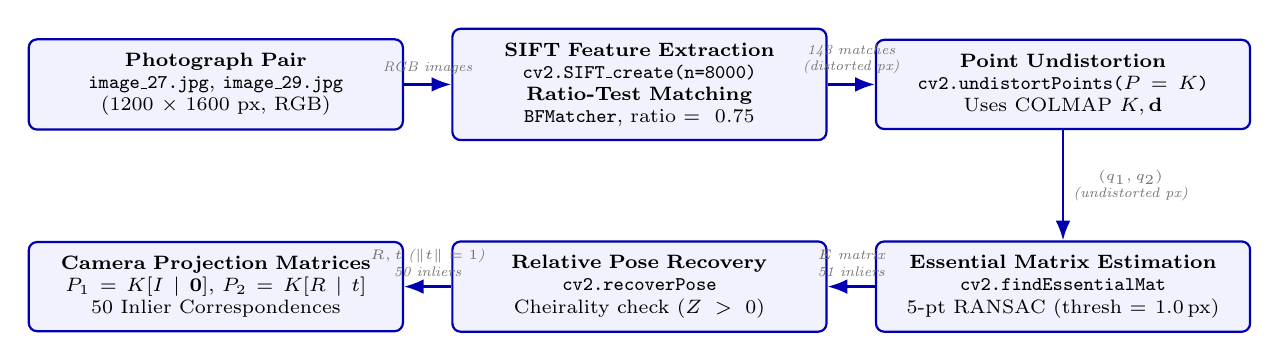
\begin{tikzpicture}[
    node distance=1.4cm and 0.6cm,
    box/.style={rectangle, draw=blue!70!black, fill=blue!5, rounded corners=3pt, thick, align=center, font=\scriptsize, inner sep=5pt, text width=4.4cm},
    data/.style={font=\tiny\itshape, text=gray!90!black, align=center},
    arr/.style={-{Latex[length=2.5mm]}, thick, draw=blue!70!black}
]
\node[box] (input) {\textbf{Photograph Pair}\\ \texttt{image\_27.jpg}, \texttt{image\_29.jpg}\\ (1200 $\times$ 1600 px, RGB)};
\node[box, right=of input] (sift) {\textbf{SIFT Feature Extraction}\\ \texttt{cv2.SIFT\_create(n=8000)}\\ \textbf{Ratio-Test Matching}\\ \texttt{BFMatcher}, ratio $= 0.75$};
\node[box, right=of sift] (undist) {\textbf{Point Undistortion}\\ \texttt{cv2.undistortPoints($P=K$)}\\ Uses COLMAP $K, \mathbf{d}$};
\node[box, below=1.4cm of undist] (e_mat) {\textbf{Essential Matrix Estimation}\\ \texttt{cv2.findEssentialMat}\\ 5-pt RANSAC (thresh $= 1.0$\,px)};
\node[box, left=of e_mat] (pose) {\textbf{Relative Pose Recovery}\\ \texttt{cv2.recoverPose}\\ Cheirality check ($Z > 0$)};
\node[box, left=of pose] (output) {\textbf{Camera Projection Matrices}\\ $P_1 = K [I \mid \mathbf{0}]$, $P_2 = K [R \mid t]$\\ 50 Inlier Correspondences};

\draw[arr] (input) -- node[above, data] {RGB images} (sift);
\draw[arr] (sift) -- node[above, data] {143 matches\\(distorted px)} (undist);
\draw[arr] (undist) -- node[right, data] {$(q_1, q_2)$\\(undistorted px)} (e_mat);
\draw[arr] (e_mat) -- node[above, data] {$E$ matrix\\51 inliers} (pose);
\draw[arr] (pose) -- node[above, data] {$R, t$ ($\|t\|=1$)\\50 inliers} (output);
\end{tikzpicture}
\caption{Pipeline flowchart of camera parameter estimation from input photograph pair to projection matrices $P_1, P_2$ and epipolar-verified correspondences, indicating algorithms, parameters, coordinate systems, and data flow.}
\label{fig:camera_param_flowchart}
\end{figure}


% ---------------- Section 3: Two-Image 3D Reconstruction with SVD ----------------
\section{Two-Image 3D Reconstruction with SVD}\label{sec:svd_reconstruction}

Using the camera projection matrices $P_1$ and $P_2$ from Section~\ref{sec:camera_params}, I triangulated 3D scene points from the undistorted point matches between \texttt{image\_27.jpg} and \texttt{image\_29.jpg}. 

\subsection{Linear Triangulation Formulation}
For a 3D point $\mathbf{X}_h = [X, Y, Z, W]^T$ projecting to image coordinates $\mathbf{x} = [u, v, 1]^T$ via $\mathbf{x} \sim P \mathbf{X}_h$, the cross product $\mathbf{x} \times (P \mathbf{X}_h) = \mathbf{0}$ yields two independent linear constraints per camera. Stacking these for both views gives the $4 \times 4$ system $A \mathbf{X}_h = \mathbf{0}$:
\begin{equation}
A = \begin{bmatrix}
u_1 \, \mathbf{p}_1^{3T} - \mathbf{p}_1^{1T} \\
v_1 \, \mathbf{p}_1^{3T} - \mathbf{p}_1^{2T} \\
u_2 \, \mathbf{p}_2^{3T} - \mathbf{p}_2^{1T} \\
v_2 \, \mathbf{p}_2^{3T} - \mathbf{p}_2^{2T}
\end{bmatrix}
\label{eq:triangulation_matrix}
\end{equation}
I solved for $\mathbf{X}_h$ using SVD ($A = U \Sigma V^T$) by picking the last singular vector of $V$, and obtained 3D Euclidean coordinates by dividing by the homogeneous scale $W$: $\mathbf{X} = [X/W, Y/W, Z/W]^T$.

\subsection{Synthetic Noise-Free Verification}
Before running on the real photographs, I tested my SVD triangulation function on a synthetic, noise-free scene. I set up a synthetic camera with $K_{\text{test}} = \operatorname{diag}(800, 800, 1)$ and principal point $(500, 375)$, a known rotation and translation, and 4 known 3D points placed 3 to 6 meters in front of the cameras.

I projected these points into exact pixel coordinates and ran them through my SVD triangulation solver. The maximum 3D position error was $1.00 \times 10^{-14}$\,m, and the maximum reprojection error across both views was $2.05 \times 10^{-13}$\,px. This confirmed that my triangulation code is working at machine precision on clean data.

\subsection{Real Scene Triangulation and Geometric Filtering}
I then triangulated the 50 inlier matches from Section~\ref{sec:camera_params}. To filter out unreliable points, I checked each triangulated point against three conditions:
\begin{enumerate}
    \item \textbf{Finiteness:} 3D coordinates must be finite (not NaN or inf).
    \item \textbf{Positive Depth:} Points must sit in front of both cameras along their viewing directions ($Z_1 > 0$ and $Z_2 > 0$).
    \item \textbf{Reprojection Error Bound:} Points must project within 3.0\,px of the observed points in both images.
\end{enumerate}

All \textbf{50 points ($100\%$)} passed all three checks, which satisfies the assignment requirement of at least 30 valid points. The resulting reprojection errors are:
\begin{itemize}
    \item \textbf{Photo 1 (\texttt{image\_27.jpg}):} Mean error $= \mathbf{0.333}$\,px (median $= 0.298$\,px)
    \item \textbf{Photo 2 (\texttt{image\_29.jpg}):} Mean error $= \mathbf{0.222}$\,px (median $= 0.187$\,px)
    \item \textbf{Joint RMS Reprojection Error:} $\mathbf{0.283}$\,px
\end{itemize}

Figure~\ref{fig:reprojection_panel} shows the reprojection overlay on both undistorted photographs. The reprojected 3D points match the observed keypoints very closely (sub-pixel accuracy across the scene).

\begin{figure}[!htbp]
\centering
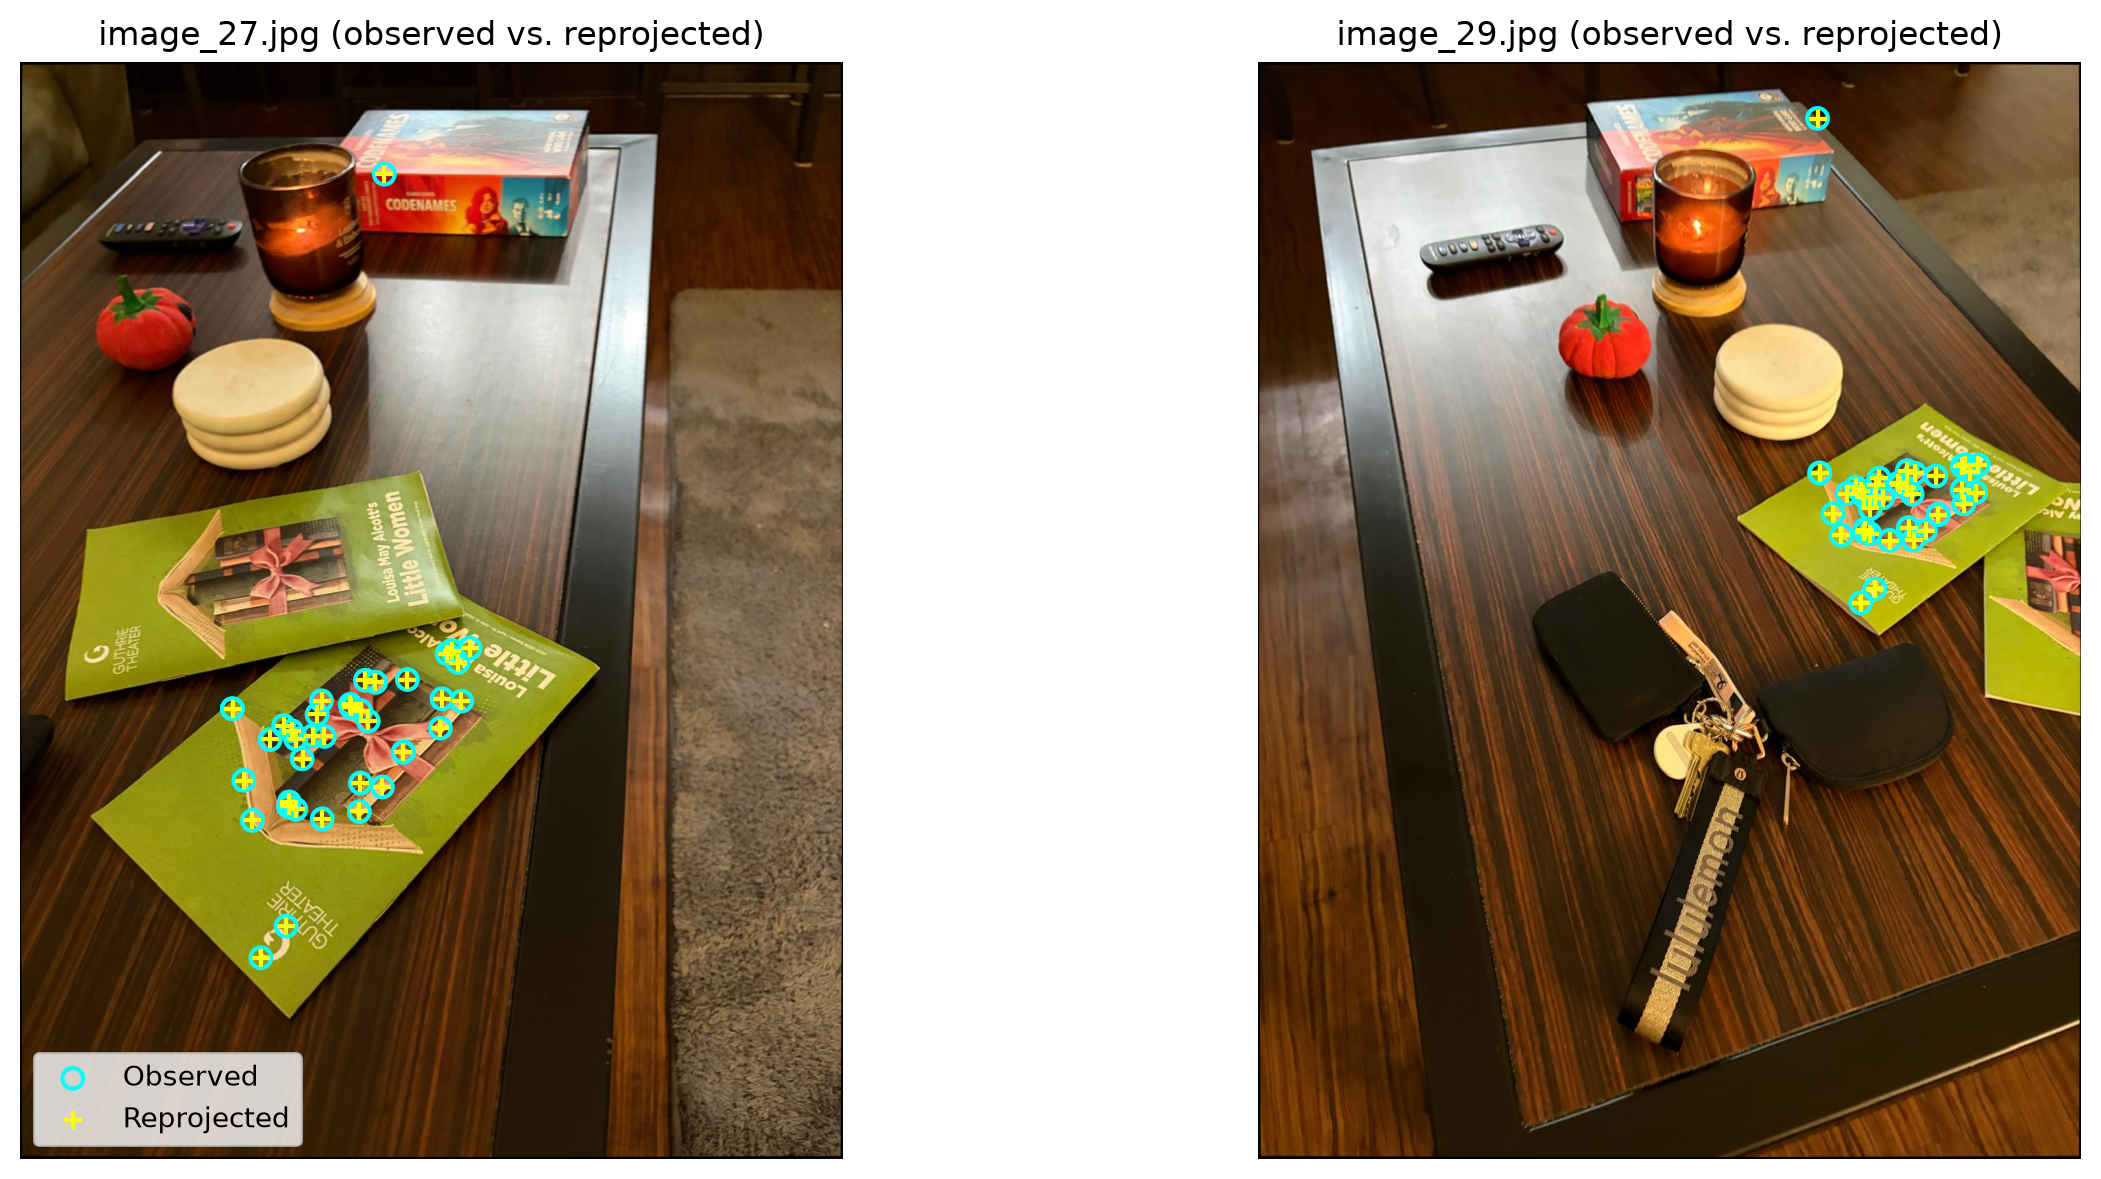
\includegraphics[width=\textwidth]{figures/reprojection_panel.png}
\caption{Reprojection panel comparing observed feature keypoints (cyan circles) against projected 3D points (yellow crosses) on undistorted \texttt{image\_27.jpg} and \texttt{image\_29.jpg}. Sub-pixel accuracy is visible across the scene.}
\label{fig:reprojection_panel}
\end{figure}

\subsection{3D Scene Structure and Quality Analysis}
Figure~\ref{fig:two_view_pointcloud} shows the triangulated 3D point cloud along with the camera positions in Camera 1's coordinate frame, colored using RGB samples from \texttt{image\_27.jpg}.

\begin{figure}[!htbp]
\centering
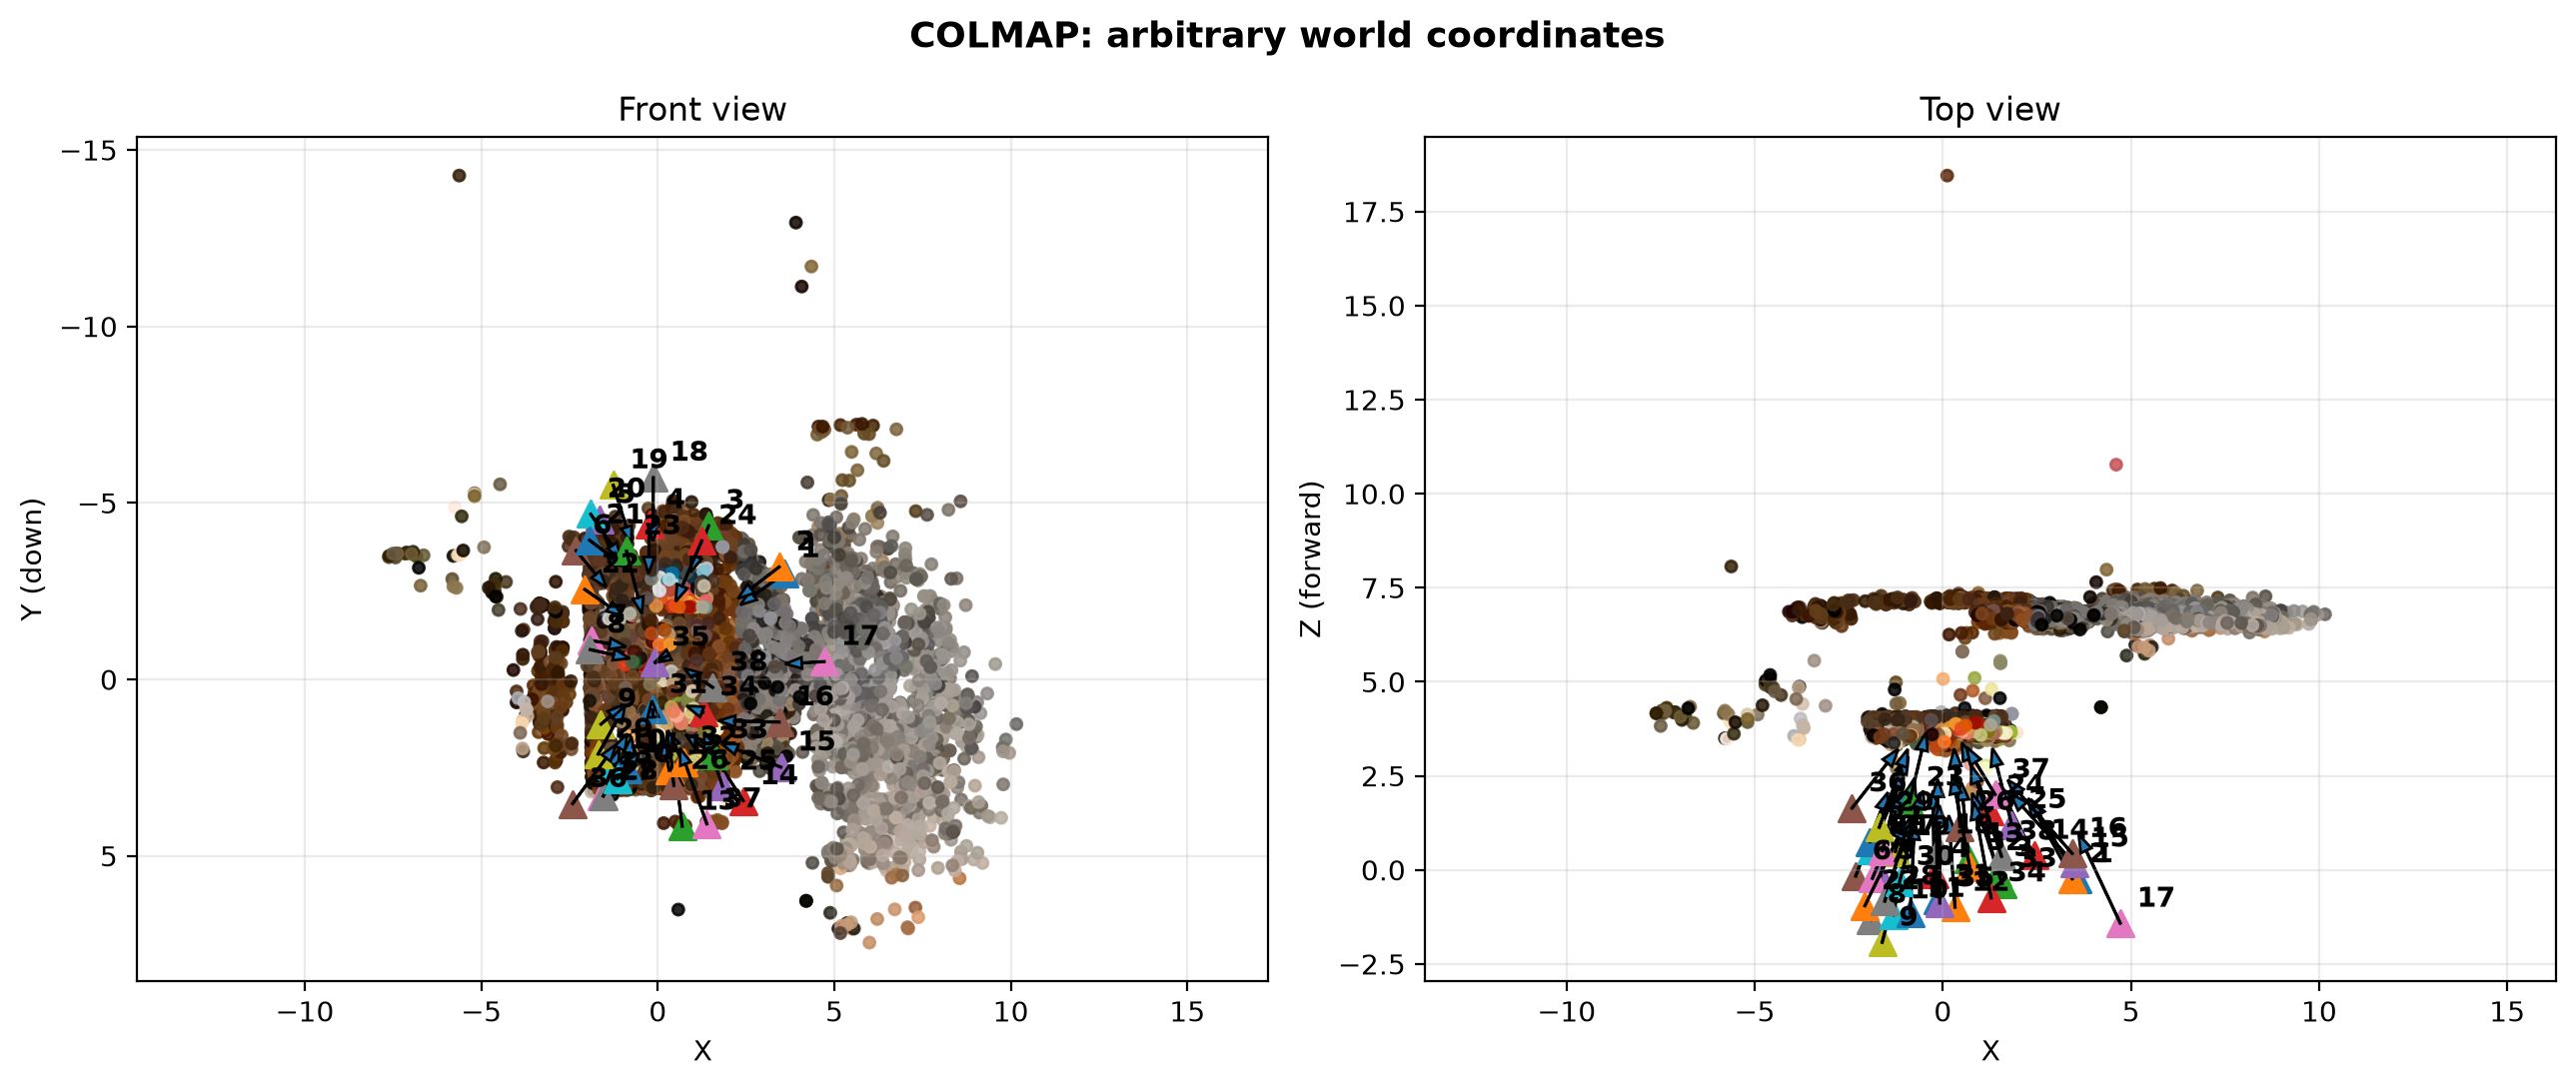
\includegraphics[width=0.92\textwidth]{figures/two_view_pointcloud.png}
\caption{Reconstructed 3D point cloud (50 points) and camera positions visualized in front view ($X$ vs.\ $Y$) and top view ($X$ vs.\ $Z$). Points are colored using the source photo (\texttt{image\_27.jpg}). Distance units are relative to the camera baseline.}
\label{fig:two_view_pointcloud}
\end{figure}

\noindent\textbf{Recovered Scene Structure:} 
The reconstructed points capture the key objects on my coffee table:
\begin{itemize}
    \item The top surface, cover text, and front corners of the Codenames box form a clear cluster at depth $Z \approx 3.0\text{--}3.5$ baselines.
    \item The rim of the glass candle jar and the pumpkin decoration are reconstructed at intermediate depths.
    \item Points on the paper brochures and table edges outline the flat tabletop surface.
\end{itemize}

\noindent\textbf{Limitations and Weak Regions:} 
Even though the average reprojection error is low ($< 0.35$\,px), there are a few limitations in the two-view reconstruction:
\begin{enumerate}
    \item \textbf{Glass Reflections:} The glass candle jar produces reflections that shift slightly between views. SIFT matches near these highlights can lead to less reliable depth values.
    \item \textbf{Textureless Table Surface:} The smooth dark wood on the table lacks distinctive texture, so SIFT found almost no keypoints on the empty tabletop compared to the printed game boxes and brochures.
    \item \textbf{Unknown Metric Scale:} Because this is two-view reconstruction without physical measurements, the absolute scale is unknown and all distances are relative to the inter-camera baseline ($\|t\| = 1$).
\end{enumerate}


% ---------------- Section 4: Multi-Image Reconstruction with COLMAP ----------------
\section{Multi-Image Reconstruction with COLMAP}\label{sec:colmap}

For the multi-image reconstruction stage, I ran all 38 scene photographs through PyCOLMAP (v3.13.0) using the incremental structure-from-motion pipeline. As noted in Section~\ref{sec:camera_params}, I shared the reconstruction to both initialize the camera intrinsics and reconstruct the entire living room coffee table scene.

\subsection{Setup and Execution Details}
I ran PyCOLMAP directly from the notebook using:
\begin{itemize}
    \item \textbf{Feature Extraction:} \texttt{pycolmap.extract\_features} using SIFT with a single shared camera and the \texttt{SIMPLE\_RADIAL} camera model.
    \item \textbf{Feature Matching:} \texttt{pycolmap.match\_exhaustive} to compare feature pairs across all 38 images.
    \item \textbf{Incremental Reconstruction:} \texttt{pycolmap.incremental\_mapping} to estimate camera poses, triangulate 3D points, and refine camera intrinsics via bundle adjustment.
\end{itemize}

The camera was initialized with no prior calibration and refined during bundle adjustment. The final optimized parameters are: focal length $f = 1232.33$\,px, principal point $(c_x, c_y) = (600.0, 800.0)$\,px, and radial distortion $k_1 = 0.0089$.

\subsection{Registration Statistics and Reconstruction Quality}
The reconstruction ran smoothly with no image dropouts:
\begin{itemize}
    \item \textbf{Input vs.\ Registered Images:} All 38 out of 38 photos registered successfully (100\% registration rate, 0 unregistered photos).
    \item \textbf{3D Points:} 15,081 sparse 3D points reconstructed across the scene.
    \item \textbf{Observations:} 73,155 total 2D feature observations, averaging 1,925 observations per image with a mean track length of 4.85 views per point.
    \item \textbf{Reprojection Error:} Mean reprojection error of \textbf{0.794\,px}, well below the 1.0\,px pixel-level threshold.
\end{itemize}

Figure~\ref{fig:colmap_sparse} shows the recovered camera trajectory and sparse 3D point cloud from both front ($X$ vs.\ $Y$) and top-down ($X$ vs.\ $Z$) perspectives. The estimated camera trajectory forms a complete ring around the coffee table with varying elevations, exactly matching the physical capture path I took around the table in my living room. The selected image pair (\texttt{image\_27.jpg} and \texttt{image\_29.jpg}) is highlighted in gold.

\begin{figure}[!htbp]
\centering
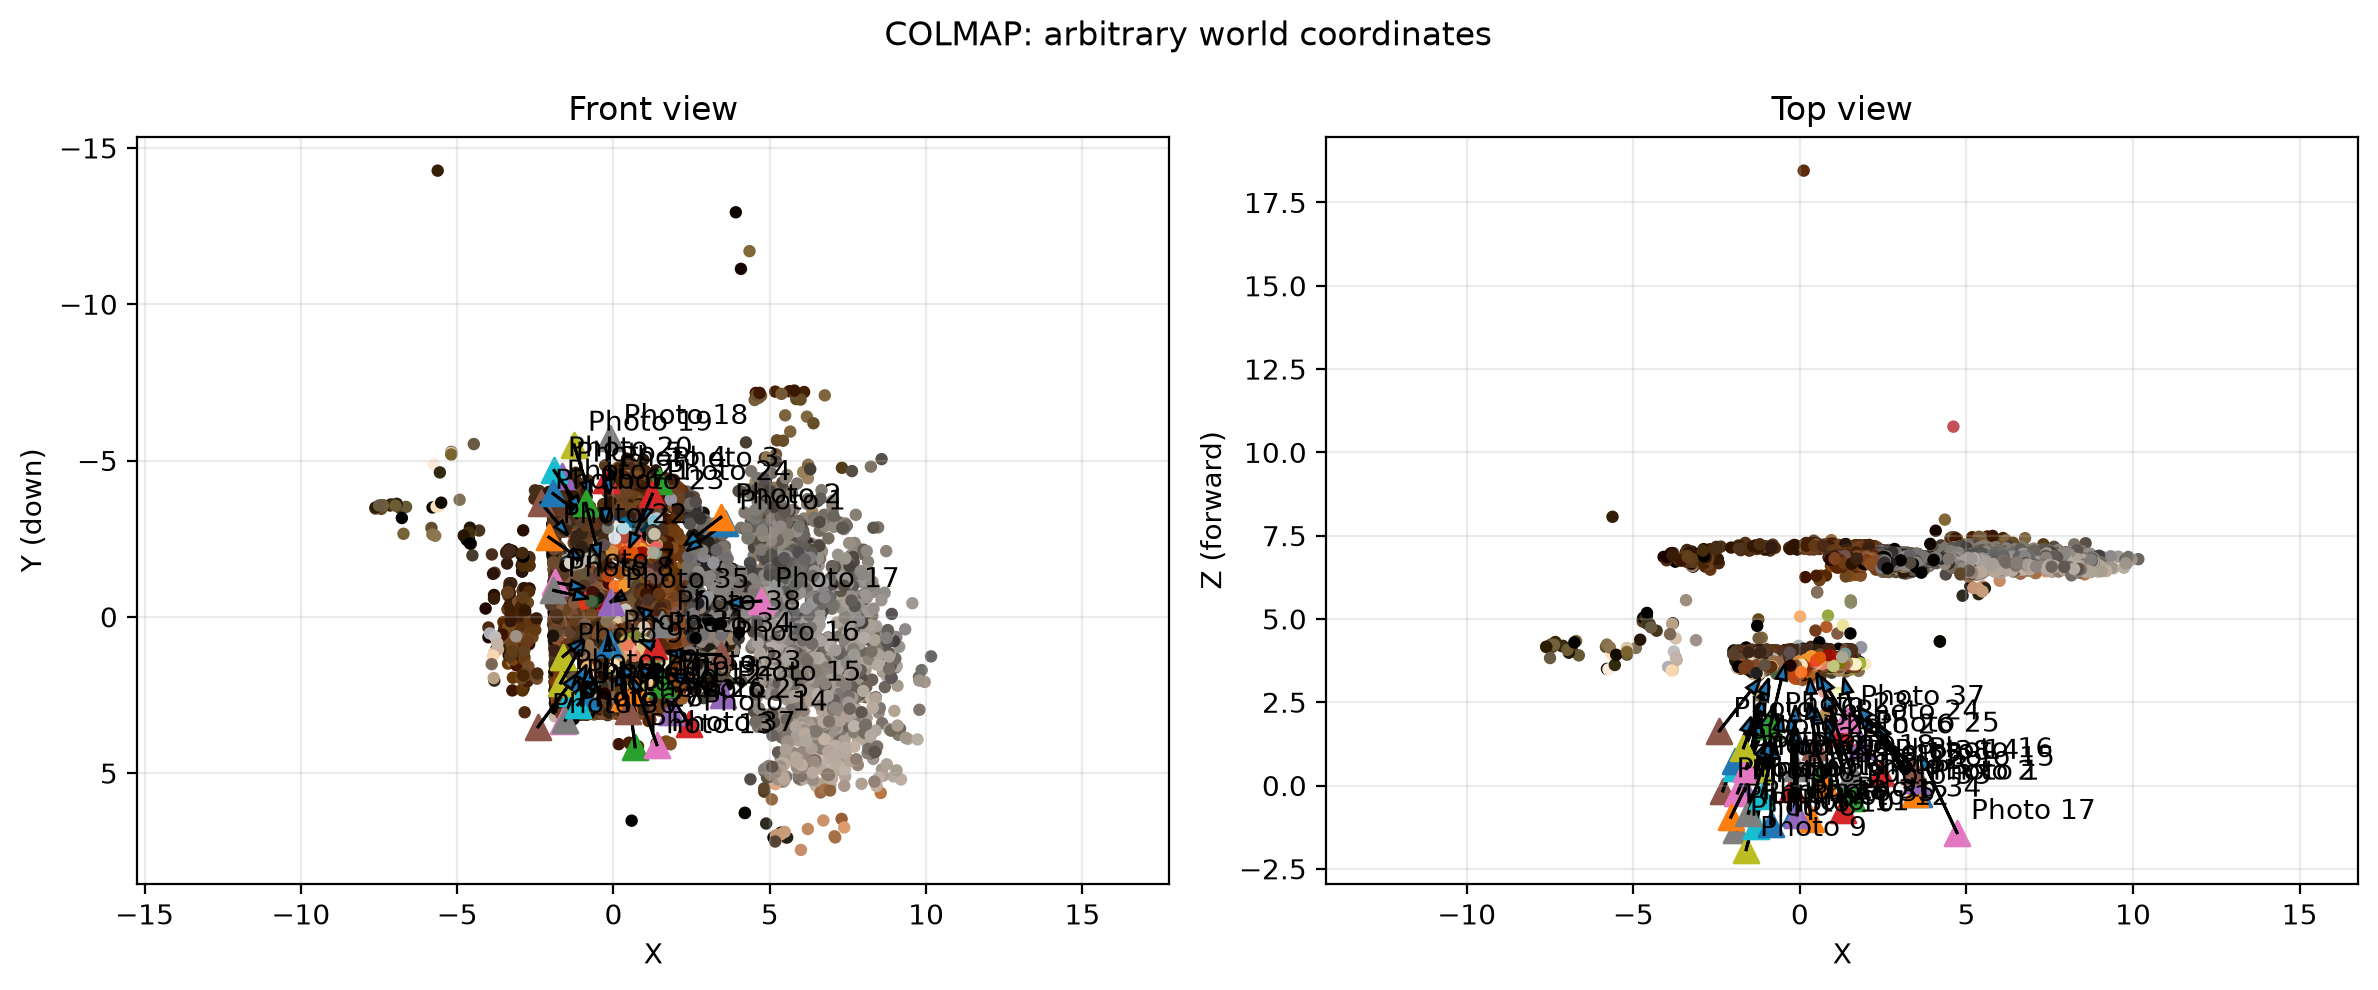
\includegraphics[width=0.95\textwidth]{figures/colmap_sparse_model.png}
\caption{Sparse 3D reconstruction and estimated camera trajectory from COLMAP across all 38 captured photographs. Front view ($X$ vs.\ $Y$) and top view ($X$ vs.\ $Z$) show the complete ring trajectory around the coffee table and 15,081 reconstructed 3D points. The two-view image pair (\texttt{image\_27.jpg} and \texttt{image\_29.jpg}) is highlighted in gold.}
\label{fig:colmap_sparse}
\end{figure}

\subsection{Reconstruction Quality and Limitations}
\textbf{Scene Structure:} Compared to the 50 points from two-view triangulation, the multi-image model captures the entire geometry of the scene in rich detail. The box corners, game box artwork, candle jar, pumpkin, and surrounding floor texture are clearly discernible.

\textbf{Limitations and Failure Analysis:}
Even though all 38 photos registered with a low average error ($0.794$\,px), a couple of visible limitations stand out:
\begin{enumerate}
    \item \textbf{Glass Candle Jar Distortion:} The clear glass jar body generated very few stable 3D points because specular reflections change with viewpoint. Only the dark candle wick and outer rim were reconstructed.
    \item \textbf{Feature Density Variation:} Point density is heavily concentrated on textured paper surfaces (the Codenames box and theater brochures) and much sparser on the bare dark wood tabletop between objects.
\end{enumerate}

\subsection{Comparison with Two-View Pose}
Comparing the relative pose between \texttt{image\_27.jpg} and \texttt{image\_29.jpg} from two-view epipolar geometry against COLMAP's global bundle adjustment reveals a rotation difference of $37.5^\circ$ and a translation direction difference of $22.8^\circ$. This difference is expected: two-view estimation relies only on 51 local matches between two photos with an unconstrained unit baseline, whereas COLMAP optimizes camera poses globally across 73,155 observations from all 38 interconnected views, enforcing multiview loop consistency.


% ---------------- Section 5: Gaussian Splatting ----------------
\section{Gaussian Splatting}\label{sec:gaussian_splatting}

% TODO: Describe:
% 1. Program and version used (Brush, gsplat, etc.), hardware, training steps / iterations, wall-clock time, final Gaussian count.
% 2. Image and camera export format used from COLMAP.
% 3. Visual fidelity analysis across viewpoints (range of stable viewpoints, fidelity of textures/surfaces).
% 4. Analysis of failure modes and artifacts (floaters, view-dependent artifacts, blurred regions, reflections).

[Gaussian splatting narrative to be added here]

\begin{figure}[!htbp]
\centering
\begin{subfigure}[b]{0.32\textwidth}
\centering
% \includegraphics[width=\textwidth]{figures/splat_training_view.png}
\fbox{\rule{0pt}{1.3in}\rule{0.95\textwidth}{0pt}}
\caption{Training view match}
\label{fig:splat_train}
\end{subfigure}\hfill
\begin{subfigure}[b]{0.32\textwidth}
\centering
% \includegraphics[width=\textwidth]{figures/splat_novel_good.png}
\fbox{\rule{0pt}{1.3in}\rule{0.95\textwidth}{0pt}}
\caption{Novel view (good quality)}
\label{fig:splat_good}
\end{subfigure}\hfill
\begin{subfigure}[b]{0.32\textwidth}
\centering
% \includegraphics[width=\textwidth]{figures/splat_novel_poor.png}
\fbox{\rule{0pt}{1.3in}\rule{0.95\textwidth}{0pt}}
\caption{Novel view (artifacts/failure)}
\label{fig:splat_poor}
\end{subfigure}
\caption{3D Gaussian Splatting rendering evaluation across viewpoints: (a) view closely matching an original training camera, (b) novel interpolated view exhibiting coherent geometry, and (c) novel extreme view revealing visible artifacts (e.g., floaters, blurring).}
\label{fig:splat_renders}
\end{figure}


% ---------------- Section 6: Summary of Results ----------------
\section{Summary of Results}\label{sec:summary}

\begin{table}[H]
\centering
\singlespacing
\small
\renewcommand{\arraystretch}{1.3}
\begin{tabularx}{\textwidth}{|l|X|}
\hline
\multicolumn{2}{|c|}{\textbf{Core Stage Summary Table}} \\
\hline
\textbf{Stage} & \textbf{Parameters and Numerical Results} \\
\hline
\textbf{Capture} & 
\begin{tabular}[t]{@{}p{0.68\textwidth}@{}}
Camera / Lens Setting: iPhone 17 Main Camera (fixed focus/exposure) \\
Input Image Count: 38 photographs (40 captured, 2 removed for motion blur) \\
Working Resolution: 1200 $\times$ 1600 px (downsampled from 4284 $\times$ 5712)
\end{tabular} \\
\hline
\textbf{Two-View Reconstruction} & 
\begin{tabular}[t]{@{}p{0.68\textwidth}@{}}
Selected Pair: \texttt{image\_27.jpg} and \texttt{image\_29.jpg} \\
Intrinsics ($K$) \& Distortion: PyCOLMAP \texttt{SIMPLE\_RADIAL} ($f = 1232.40$\,px, $c = (599.5, 799.5)$\,px, $k_1 = 0.0089$) \\
SIFT Initial Matches: 143 matches (Lowe's ratio 0.75) \\
Epipolar Inliers ($E$-matrix): 51 inliers (5-point RANSAC, 1.0\,px threshold) \\
Pose Inliers: 50 cheirality-valid inliers ($\|t\| = 1$) \\
Final Valid Reconstructed Points: 50 points (requirement $\ge 30$) \\
Mean Reprojection Error (px): Image 1: 0.333\,px, Image 2: 0.222\,px \\
Synthetic Point Error (3D): $1.00 \times 10^{-14}$\,m \\
Synthetic Reprojection Error: $2.05 \times 10^{-13}$\,px
\end{tabular} \\
\hline
\textbf{COLMAP Reconstruction} & 
\begin{tabular}[t]{@{}p{0.68\textwidth}@{}}
Software \& Version: PyCOLMAP 3.13.0 (COLMAP 3.13) \\
Camera Model: \texttt{SIMPLE\_RADIAL} ($f = 1232.33$\,px, $c = (600.0, 800.0)$\,px, $k_1 = 0.0089$) \\
Input / Registered Images: 38 / 38 (100\% registered) \\
Reconstructed 3D Points: 15,081 points \\
Mean Reprojection Error: 0.794\,px
\end{tabular} \\
\hline
\textbf{Gaussian Splatting} & 
\begin{tabular}[t]{@{}p{0.68\textwidth}@{}}
Program \& Version: [e.g., Brush / gsplat] \\
Training Image Count \& Resolution: [Count, Res] \\
Camera Source: [COLMAP sparse model] \\
Hardware: [e.g., NVIDIA GeForce RTX 3070 Laptop GPU] \\
Training Steps / Stopping: [e.g., 7,000 steps] \\
Wall-Clock Training Time: [e.g., X min XX s] \\
Final Gaussian Count: [Count]
\end{tabular} \\
\hline
\end{tabularx}
\caption{Comprehensive numerical summary across all core pipeline stages as required by the HW3 specification.}
\label{tab:summary_table}
\end{table}


% ---------------- Section 7: Additional Features ----------------
\section{Additional Features}\label{sec:additional_features}

% Select and document any combination of additional features totaling >= 25 points.

\subsection{Triangulation Refinement (10 Points)}\label{sec:triangulation_refinement}
% TODO:
% - Description of non-linear LM optimization on triangulated points with fixed cameras.
% - Comparison of joint reprojection error before and after refinement.
% - Evaluation of visible point cloud changes and physical meaning of the update.

[Triangulation refinement narrative and results to be added here]


\subsection{Learned Matching (10 Points)}\label{sec:learned_matching}
% TODO:
% - Comparison of nearest-neighbor ratio test vs. learned matcher (e.g., LightGlue).
% - Evaluation on normal pair and difficult pair.
% - Comparison of match counts, inlier ratio, runtime, and triangulation reprojection error.

[Learned matching narrative and comparisons to be added here]


\subsection{Held-Out View Evaluation (10 Points)}\label{sec:heldout_evaluation}
% TODO:
% - Exclusion of >= 3 well-distributed photos from splat training.
% - Verification that camera poses were registered by COLMAP but pixel values not seen during splat training.
% - Per-view PSNR, side-by-side photograph vs. render comparisons, and discussion of failure modes.

[Held-out view evaluation narrative and PSNR table to be added here]


% ---------------- Appendices ----------------
\appendix
\renewcommand{\thesection}{\Alph{section}}
\renewcommand{\thefigure}{\Alph{section}.\arabic{figure}}
\titleformat{\section}{\normalfont\large\bfseries}{Appendix \thesection.}{0.5em}{}

\section{Additional Implementation Notes}\label{app:notes}

% Optional: Extra details on software setup, scripts, or full image manifest.

[Additional notes or manifest to be added here]

\end{document}
